\documentclass[a4paper]{article}
\title{SmartFolder}
\author{Maxime Lovino \and Thomas Ibanez}
\usepackage[francais]{babel}
\usepackage{fontspec}
\usepackage{pgfplots}
\pgfplotsset{width=10cm,compat=1.9}
% \setmainfont{Helvetica Neue}
\usepackage{amsmath}
\usepackage{amsfonts}
\usepackage{xcolor,graphicx}
\definecolor{light-gray}{gray}{0.95}
\usepackage{minted}
\usemintedstyle{colorful}
\setlength{\parindent}{0pt}
\usepackage[left=2.5cm,top=2.5cm,right=2.5cm,bottom=2.5cm]{geometry}
\begin{document}
\maketitle
\newpage
\section{Introduction}
Hello world
\section{Architecture}
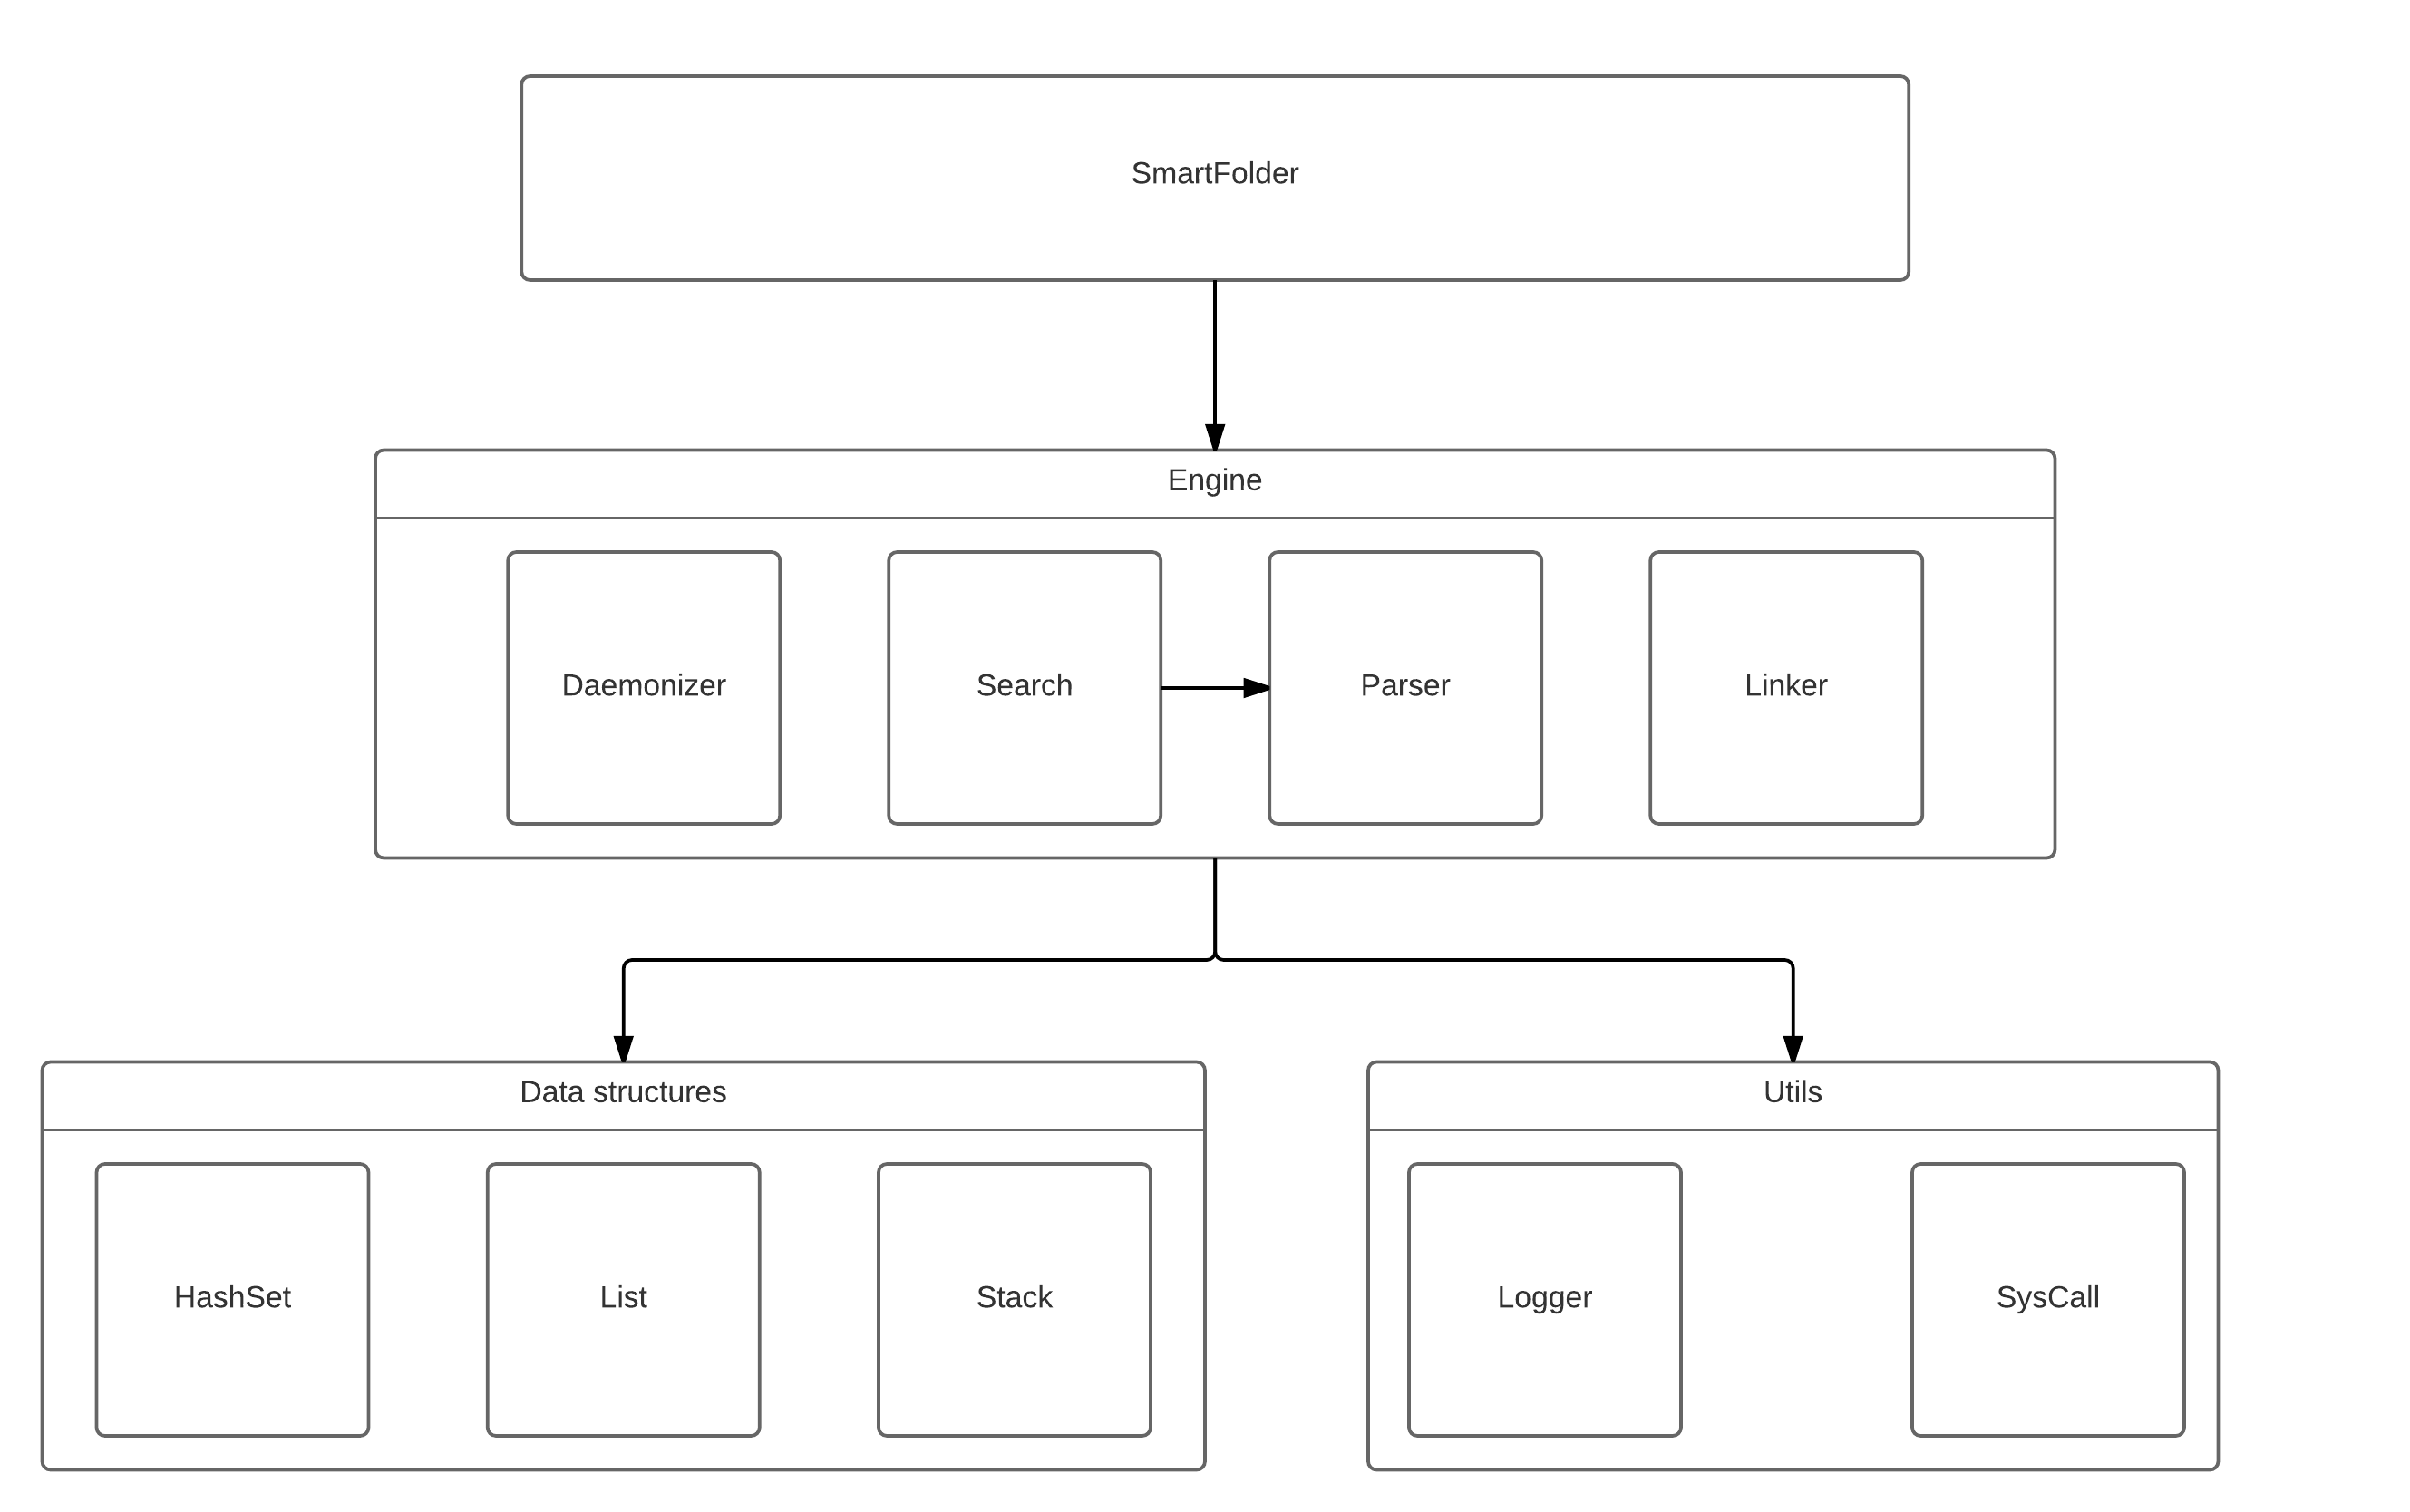
\includegraphics[width=\textwidth]{diagram.png}
\subsection{Data Structures}
\subsubsection{List}
Nous avons une structure de liste qui sert à stocker la liste des résultats d'une recherhe (liste de fichiers). Nous définissions des fonctions permettant d'agréer plusieurs listes au travers d'une union, intersection, etc... correspondant aux opérations booléennes classiques.
\inputminted[breaklines,breaksymbol=, frame=single, stepnumber=5,tabsize=2]{C}{../src/List.h}
\subsubsection{HashSet}
Nous avons une structure de table de hachage permettant de stocker les matches actuels présent dans le dossier, cela nous permet lors du prochain run de la recherche de tester de façon rapide (recherche en $O(1)$ en général et maximum en $\Theta(n)$).
\inputminted[breaklines,breaksymbol=, frame=single, stepnumber=5,tabsize=2]{C}{../src/HashSet.h}
\subsubsection{Stack}
Nous utilisons une structure de Pile pour stocker les résultats d'une recherche particulière (on stocke un pointeur de la liste des résultats) pour ensuite les rassembler lorsque nous trouvons un opérateur booléen. (principe de l'évaluation d'une expression polonaise inverse)
\inputminted[breaklines,breaksymbol=, frame=single, stepnumber=5,tabsize=2]{C}{../src/Stack.h}
\subsection{Utils}
\subsubsection{Logger}
\subsubsection{SysCall}
\subsection{Engine}
\subsubsection{Search}
\subsubsection{Parser}
\subsubsection{Linker}
\subsubsection{Daemonizer}
\subsection{SmartFolder}








\end{document}
